\numoptsfalse
\yearpaper{2021}{Version A1 \textperiodcentered{} 60 Questions \textperiodcentered{} 60 Marks \textperiodcentered{} 80 Minutes}{}
\begin{multicols}{2}

\QQ{For a body moving along a straight line, the following v-t graph is obtained.
\fig{\begin{tikzpicture}[scale=0.75]
\draw[->] (-0.3,0) -- (3.6,0) node[right,lbl]{$t$ (s)};
\draw[->] (0,-0.2) -- (0,2.3) node[above,lbl]{$v$ (m/s)};
\draw (0,0.8) -- (1.0,1.7) -- (2.8,1.7);
\draw[densely dashed] (1.0,1.7) -- (1.0,0) (2.8,1.7) -- (2.8,0);
\end{tikzpicture}}
According to the graph, the displacement during}
{\opt{Uniform acceleration is greater than that during uniform motion.}{Uniform acceleration is less than that during uniform motion.}{Uniform acceleration is equal to that during uniform motion.}{Uniform motion is zero.}}

\QQ{A particle starts from rest. Its acceleration `$a$' versus time `$t$' is shown in the figure. The maximum speed of the particle will be:
\fig{\begin{tikzpicture}[scale=0.75]
\draw[->] (0,0) -- (2.8,0) node[right,lbl]{$t$ (s)};
\draw[->] (0,0) -- (0,2.0) node[above,lbl]{$a$ (m\,s$^{-2}$)};
\draw (0,1.6) -- (2.0,0);
\node[lbl,left] at (0,1.6) {8}; \node[lbl,below] at (2.0,0) {10}; \node[lbl,below left] at (0,0) {0};
\end{tikzpicture}}}
{\opt{$80\unit{m\,s^{-1}}$}{$40\unit{m\,s^{-1}}$}{$18\unit{m\,s^{-1}}$}{$2\unit{m\,s^{-1}}$}}

\QQ{The maximum range of a gun on horizontal plane is $16\unit{km}$. If $g = 10\unit{m\,s^{-2}}$, then muzzle velocity of a shell is}
{\opt{$160\unit{m\,s^{-1}}$}{$200\sqrt2\unit{m\,s^{-1}}$}{$400\unit{m\,s^{-1}}$}{$800\unit{m\,s^{-1}}$}}

\QQ{The trajectory of a projectile is}
{\opt{semicircle}{an ellipse}{a parabola always}{a parabola in the absence of air resistance}}

\QQ{For a projectile motion, the angle between the velocity and acceleration is minimum and acute at}
{\opt{only one point}{two points}{three points}{four points}}

\QQ{A particle starts from the origin at $t = 0\unit{s}$ with a velocity of $10\hat j\unit{m\,s^{-1}}$ and moves in the $x$-$y$ plane with a constant acceleration of $(8\hat i+2\hat j)\unit{m\,s^{-2}}$. At an instant when the $x$-coordinate of the particle is $16\unit{m}$, $y$-coordinate of the particle is:}
{\opt{$16\unit{m}$}{$28\unit{m}$}{$36\unit{m}$}{$24\unit{m}$}}

\QQ{A coin placed on a rotating turn table just slips if it is placed at a distance of $4\unit{cm}$ from the centre. If the angular velocity of the turn table is doubled it will just slip at a distance of:}
{\opt{$1\unit{cm}$}{$2\unit{cm}$}{$4\unit{cm}$}{$8\unit{cm}$}}

\QQ{A $1\unit{kg}$ ball moving at $12\unit{m\,s^{-1}}$ collides with a $2\unit{kg}$ ball moving in opposite direction at $24\unit{m\,s^{-1}}$. If the coefficient of restitution is $\frac23$, then their velocities after the collision are}
{\opt{$-4\unit{m\,s^{-1}}$, $-28\unit{m\,s^{-1}}$}{$-28\unit{m\,s^{-1}}$, $-4\unit{m\,s^{-1}}$}{$4\unit{m\,s^{-1}}$, $28\unit{m\,s^{-1}}$}{$28\unit{m\,s^{-1}}$, $4\unit{m\,s^{-1}}$}}

\QQ{A ball hits the floor and rebounds after an inelastic collision. In this case}
{\opt{the momentum of the ball is conserved}{the mechanical energy of the ball is conserved}{the total momentum of the ball and the earth is conserved}{the total mechanical energy of the ball and the earth is conserved}}

\QQ{In figure $E$ and $V_{cm}$ represent the total energy and speed of centre of mass of an object of mass $1\unit{kg}$ in pure rolling. The object is:
\fig{\begin{tikzpicture}[scale=0.75]
\draw[->] (0,0) -- (3.0,0) node[right,lbl]{$V^2_{cm}$ (m$^2$s$^{-2}$)};
\draw[->] (0,0) -- (0,2.4) node[above,lbl]{$E$ (J)};
\draw (0,0) -- (2.2,2.1);
\draw[densely dotted] (0,1.5) node[left,lbl]{3} -- (1.57,1.5) -- (1.57,0) node[below,lbl]{4};
\node[lbl,below left] at (0,0) {0};
\end{tikzpicture}}}
{\opt{sphere}{ring}{disc}{Hollow Cylinder}}

\QQ{Two bodies of masses $8\unit{kg}$ are placed at the vertices A and B of an equilateral triangle ABC. A third body of mass $2\unit{kg}$ is placed at the centroid G of the triangle. If $AG = BG = CG = 1\unit{m}$, where should a fourth body of mass $4\unit{kg}$ be placed so that the resultant force on the $2\unit{kg}$ body is zero?}
{\opt{at C}{at a point P on the line CG such that $PG = \dfrac{1}{\sqrt2}\unit{m}$}{at a point P on the line CG such that $PG = 0.5\unit{m}$}{at a point P on the line CG such that $PG = 2\unit{m}$}}

\QQ{Two capillary tubes P and Q are dipped vertically in water. The height of water level in capillary tube P is $\frac23$rd of the height in capillary tube Q. The ratio of their diameter is \rule{1.2cm}{0.4pt}.}
{\opt{2:3}{3:2}{3:4}{4:3}}

\QQ{Which of the following curves represent the variation of coefficient of volume expansion of an ideal gas at constant pressure?}
{\optfig{\gaxes{$T$}{$\alpha_v$}{\draw (0.3,0.2) -- (1.6,1.5);}}
{\gaxes{$\frac1T$}{$\alpha_v$}{\draw (0.3,0.2) -- (1.6,1.5);}}
{\gaxes{$\frac1T$}{$\alpha_v$}{\draw (0.2,1.0) -- (1.8,1.0);}}
{\gaxes{$T$}{$\alpha_v$}{\draw (0.4,1.5) -- (1.8,0.3);}}}

\QQ{A number of Carnot engines are operated at identical cold reservoir temperatures ($T_L$). However, their hot reservoir temperatures are kept different. A graph of the efficiency of the engines versus hot reservoir temperature ($T_H$) is plotted. The correct graphical representation is}
{\optfig{\gaxes{$T_H$}{$\eta$}{\draw[densely dotted] (0.5,0) node[below,lbl]{$T_L$} -- (0.5,1.4); \draw (0.5,1.4) .. controls (1.1,1.4) and (1.4,0.7) .. (1.6,0);}}
{\gaxes{$T_H$}{$\eta$}{\draw[densely dotted] (0.5,0) node[below,lbl]{$T_L$} -- (0.5,1.4); \draw (0.5,0) .. controls (0.8,0.9) and (1.2,1.4) .. (1.9,1.5);}}
{\gaxes{$T_H$}{$\eta$}{\draw[densely dotted] (0.5,0) node[below,lbl]{$T_L$} -- (0.5,1.4); \draw (0.5,0) -- (1.8,1.4);}}
{\gaxes{$T_H$}{$\eta$}{\draw[densely dotted] (1.2,0) node[below,lbl]{$T_L$} -- (1.2,1.4); \draw (0,1.5) .. controls (0.6,1.4) and (1.0,0.8) .. (1.2,0);}}}

\QQ{A gas mixture contains monoatomic and diatomic molecules of 2 moles each. The mixture has a total internal energy of (symbols have usual meanings)}
{\opt{$3RT$}{$5RT$}{$8RT$}{$9RT$}}

\QQ{A pendulum oscillates simple harmonically if and only if
\begin{stmts}[(\Roman*)]
\item the size of the bob of pendulum is negligible in comparison with the length of the pendulum.
\item the angular amplitude is less than $10^\circ$.
\end{stmts}}
{\opt{Both (I) and (II) are correct}{Both (I) and (II) are incorrect}{Only (I) is correct}{Only (II) is correct}}

\QQ{To propagate both longitudinal and transverse waves, a material must have}
{\opt{Bulk and shear moduli}{Only bulk modulus}{Only shear modulus}{Young's and Bulk modulus}}

\QQ{A copper rod AB of length $l$ is rotated about end A with a constant angular velocity $\omega$. The electric field at a distance $x$ from the axis of rotation is}
{\opt{$\dfrac{m\omega^2x}{e}$}{$\dfrac{m\omega x}{el}$}{$\dfrac{mx}{\omega^2l}$}{$\dfrac{me}{\omega^2x}$}}

\QQ{Electric field due to infinite, straight uniformly charged wire varies with distance `$r$' as}
{\opt{$r$}{$\dfrac1r$}{$\dfrac1{r^2}$}{$r^2$}}

\QQ{A 2-gram object, located in a region of uniform electric field $\vec E = (300\unit{N\,C^{-1}})\,\hat i$ carries a charge $Q$. The object released from rest at $x = 0$, has a kinetic energy of $0.12\unit{J}$ at $x = 0.5\unit{m}$. Then $Q$ is}
{\opt{$400\unit{\mu C}$}{$-400\unit{\mu C}$}{$800\unit{\mu C}$}{$-800\unit{\mu C}$}}

\QQ{If a slab of insulating material (conceptual) $4\times10^{-3}\unit{m}$ thick is introduced between the plates of a parallel plate capacitor, the separation between the plates has to be increased by $3.5\times10^{-3}\unit{m}$ to restore the capacity to original value. The dielectric constant of the material will be}
{\opt{6}{8}{10}{12}}

\QQ{Eight drops of mercury of equal radii combine to form a big drop. The capacitance of a bigger drop as compared to each smaller drop is}
{\opt{2 times}{8 times}{4 times}{16 times}}

\QQ{Which of the statements is false in the case of polar molecules?}
{\opt{Centers of positive and negative charges are separated in the absence of external electric field.}{Centers of positive and negative charges are separated in the presence of external electric field.}{Do not possess permanent dipole moments.}{Ionic molecule HCl is the example of polar molecule.}}

\QQ{An electrician requires a capacitance of $6\unit{\mu F}$ in a circuit across a potential difference of $1.5\unit{kV}$. A large number of $2\unit{\mu F}$ capacitors which can withstand a potential difference of not more than $500\unit{V}$ are available. The minimum number of capacitors required for the purpose is}
{\opt{3}{9}{6}{27}}

\QQ{In figure, charge on the capacitor is plotted against potential difference across the capacitor. The capacitance and energy stored in the capacitor are respectively.
\fig{\begin{tikzpicture}[scale=0.75]
\draw[->] (0,0) -- (2.8,0) node[right,lbl]{$V$ (volt)};
\draw[->] (0,0) -- (0,2.3) node[above,lbl]{$Q$ ($\mu$C)};
\draw (0,0) -- (1.5,1.6);
\draw[densely dotted] (0,1.6) node[left,lbl]{120} -- (1.5,1.6) -- (1.5,0) node[below,lbl]{10 V};
\node[lbl,below left] at (0,0) {0};
\end{tikzpicture}}}
{\opt{$12\unit{\mu F}$, $1200\unit{\mu J}$}{$12\unit{\mu F}$, $600\unit{\mu J}$}{$24\unit{\mu F}$, $600\unit{\mu J}$}{$24\unit{\mu F}$, $1200\unit{\mu J}$}}

\QQ{A wire of resistance $3\unit{\Omega}$ is stretched to twice its original length. The resistance of the new wire will be}
{\opt{$1.5\unit{\Omega}$}{$3\unit{\Omega}$}{$6\unit{\Omega}$}{$12\unit{\Omega}$}}

\QQ{In the given arrangement of experiment on metre bridge, if AD corresponding to null deflection of the galvanometer is X, what would be its value if the radius of the wire AB is doubled?
\fig{\begin{circuitikz}[scale=0.6,transform shape,font=\Large]
\draw (0,0) node[below]{A} -- (6,0) node[below]{B};
\draw (0,0) -- (0,2.2) to[R,l=$R_1$] (3,2.2) to[R,l=$R_2$] (6,2.2) -- (6,0);
\draw (0,2.2) -- (0,3.6) -- (2.5,3.6) to[battery1] (3.5,3.6) -- (6,3.6) -- (6,2.2);
\draw (3,2.2) to[rmeter,t=G] (2.6,0);
\node[below] at (2.6,0) {D};
\draw[<->] (0.2,-0.6) -- (2.4,-0.6) node[midway,below]{$x$};
\end{circuitikz}}}
{\opt{X}{$\dfrac X4$}{4X}{2X}}

\QQ{A copper wire of length $1\unit{m}$ and uniform cross-sectional area $5\times10^{-7}\unit{m^2}$ carries a current of $1\unit{A}$. Assuming that there are $8\times10^{28}$ free electrons per $\mathrm{m^3}$ in copper, how long will an electron take to drift from one end of the wire to the other?}
{\opt{$0.8\times10^3\unit{s}$}{$1.6\times10^3\unit{s}$}{$3.2\times10^3\unit{s}$}{$6.4\times10^3\unit{s}$}}

\QQ{Consider an electrical conductor connected across a potential difference $V$. Let $\Delta q$ be a small charge moving through it in time $\Delta t$. If $I$ is the electric current through it,
\begin{stmts}[(\Roman*)]
\item the kinetic energy of the charge increases by $IV\Delta t$.
\item the electric potential energy of the charge decreases by $IV\Delta t$.
\item the thermal energy of the conductor increases by $IV\Delta t$.
\end{stmts}
Then the correct statement/s is / are}
{\opt{(I)}{(I), (II)}{(I) and (III)}{(II), (III)}}

\QQ{A strong magnetic field is applied on a stationary electron. Then the electron}
{\opt{Moves in the direction of the field}{Moves in an opposite direction of the field}{Remains stationary}{Starts spinning}}

\QQ{Two parallel wires in free space are $10\unit{cm}$ apart and each carries a current of $10\unit{A}$ in the same direction. The force exerted by one wire on the other [per unit length] is}
{\opt{$2\times10^{-4}\unit{N\,m^{-1}}$ [attractive]}{$2\times10^{-7}\unit{N\,m^{-1}}$ [attractive]}{$2\times10^{-4}\unit{N\,m^{-1}}$ [repulsive]}{$2\times10^{-7}\unit{N\,m^{-1}}$ [repulsive]}}

\QQ{A toroid with thick windings of $N$ turns has inner and outer radii $R_1$ and $R_2$ respectively. If it carries certain steady current $I$, the variation of the magnetic field due to the toroid with radial distance is correctly graphed in}
{\optfig{\gaxes{$r$}{$B$}{\draw (0,0) -- (0.8,1.3) .. controls (1.0,1.0) and (1.2,0.9) .. (1.4,0.85) -- (1.4,0); \draw[densely dotted] (0,1.3) node[left,font=\tiny]{$\frac{\mu_0NI}{2R_1}$} -- (0.8,1.3) (0,0.85) node[left,font=\tiny]{$\frac{\mu_0NI}{2R_2}$} -- (1.4,0.85); \node[font=\tiny,below] at (0.8,0) {$R_1$}; \node[font=\tiny,below] at (1.4,0) {$R_2$};}}
{\gaxes{$r$}{$B$}{\draw (0,0) -- (0.8,1.3) .. controls (1.0,1.0) and (1.2,0.9) .. (1.4,0.85) -- (1.4,0); \draw[densely dotted] (0,1.3) node[left,font=\tiny]{$\frac{\mu_0NI}{2\pi R_1}$} -- (0.8,1.3) (0,0.85) node[left,font=\tiny]{$\frac{\mu_0NI}{2\pi R_2}$} -- (1.4,0.85); \node[font=\tiny,below] at (0.8,0) {$R_1$}; \node[font=\tiny,below] at (1.4,0) {$R_2$};}}
{\gaxes{$r$}{$B$}{\draw (0.8,0.7) .. controls (1.1,0.75) and (1.35,0.9) .. (1.4,1.3) -- (1.4,0); \draw (0.8,0.7) -- (0.8,0); \draw[densely dotted] (0,1.3) node[left,font=\tiny]{$\frac{\mu_0NI}{2\pi R_2}$} -- (1.4,1.3) (0,0.7) node[left,font=\tiny]{$\frac{\mu_0NI}{2\pi R_1}$} -- (0.8,0.7); \node[font=\tiny,below] at (0.8,0) {$R_1$}; \node[font=\tiny,below] at (1.4,0) {$R_2$};}}
{\gaxes{$r$}{$B$}{\draw (0,0) -- (0.8,0) -- (0.8,0.9) -- (1.5,0.9) -- (1.5,0); \draw[densely dotted] (0,0.9) node[left,font=\tiny]{$\frac{\mu_0NI}{\pi(R_1+R_2)}$} -- (0.8,0.9);}}}

\QQ{A tightly wound long solenoid has `$n$' turns per unit length, a radius `$r$' and carries a current $I$. A particle having charge `$q$' and mass `$m$' is projected from a point on the axis in a direction perpendicular to the axis. The maximum speed of the particle for which the particle does not strike the solenoid is}
{\opt{$\dfrac{\mu_0nIqr}{m}$}{$\dfrac{\mu_0nIqr}{2m}$}{$\dfrac{\mu_0nIqr}{4m}$}{$\dfrac{\mu_0nIqr}{8m}$}}

\QQ{Earth's magnetic field always has a horizontal component except at}
{\opt{equator}{magnetic poles}{a latitude of $60^\circ$}{an altitude of $60^\circ$}}

\QQ{Which of the field pattern given below is valid for electric field as well as for magnetic field?}
{\optfig{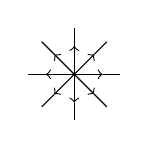
\begin{tikzpicture}[scale=0.45]\foreach \a in {0,45,...,315} \draw[->] (0,0) -- (\a:0.8); \foreach \a in {0,45,...,315} \draw (\a:0.8) -- (\a:1.3);\end{tikzpicture}}
{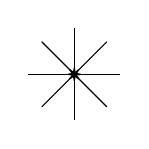
\begin{tikzpicture}[scale=0.45]\foreach \a in {0,45,...,315} \draw[<-] (0,0) -- (\a:0.8); \foreach \a in {0,45,...,315} \draw (\a:0.8) -- (\a:1.3);\end{tikzpicture}}
{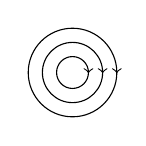
\begin{tikzpicture}[scale=0.45]\foreach \r in {0.45,0.85,1.25} {\draw (0,0) circle (\r); \draw[->] (\r,0.02) -- (\r,-0.02);}\end{tikzpicture}}
{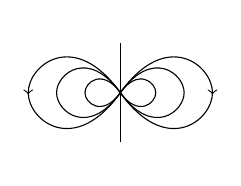
\begin{tikzpicture}[scale=0.45]\foreach \s in {0.5,0.9,1.3} {\draw (0,0) .. controls (\s,1.4*\s) and (2*\s,0.6*\s) .. (2*\s,0) .. controls (2*\s,-0.6*\s) and (\s,-1.4*\s) .. (0,0); \draw (0,0) .. controls (-\s,1.4*\s) and (-2*\s,0.6*\s) .. (-2*\s,0) .. controls (-2*\s,-0.6*\s) and (-\s,-1.4*\s) .. (0,0);} \draw (0,-1.4) -- (0,1.4); \draw[->] (2.6,0.05) -- (2.6,-0.05); \draw[->] (-2.6,0.05) -- (-2.6,-0.05);\end{tikzpicture}}}

\QQ{The current flowing through an inductance coil of self inductance $6\unit{mH}$ at different time instants is as shown. The emf induced between $t = 20\unit{s}$ and $t = 40\unit{s}$ is nearly
\fig{\begin{tikzpicture}[xscale=0.045,yscale=0.42]
\draw[->] (0,0) -- (55,0) node[right,lbl]{$t$ (s)};
\draw[->] (0,0) -- (0,5.2) node[above,lbl]{$I$ (A)};
\draw (0,0) -- (20,4.6) -- (40,3.6) -- (50,0);
\draw (20,0) -- (20,4.6) (40,0) -- (40,3.6);
\foreach \y in {2,4} {\draw (0.8,\y) -- (-0.8,\y) node[left,lbl]{\y};}
\node[lbl,below] at (20,0) {20}; \node[lbl,below] at (40,0) {40};
\end{tikzpicture}}}
{\opt{$2\times10^{-2}\unit{V}$}{$3\times10^{-2}\unit{V}$}{$4\times10^{-3}\unit{V}$}{$30\times10^{2}\unit{V}$}}

\QQ{The physical quantity which is measured in the unit of $\mathrm{Wb\,A^{-1}}$ is}
{\opt{Self inductance}{Mutual inductance}{Magnetic flux}{Both (A) and (B)}}

\QQ{What will be the reading in the voltmeter and ammeter of the circuit shown?
\fig{\begin{circuitikz}[scale=0.6,transform shape,font=\Large]
\draw (0,3) -- (3,3) to[rmeter,t=A] (6,3) to[sV,l=$90\,\mathrm{V}$] (6,0) to[R,l={$R=45\,\Omega$}] (3,0) to[L,l={$X_L=4\,\Omega$}] (0,0) to[C,l={$X_C=4\,\Omega$}] (0,3);
\draw (3,3) to[rmeter,t=V] (3,0);
\end{circuitikz}}}
{\opt{90\,V, 2\,A}{0\,V, 2\,A}{90\,V, 1\,A}{0\,V, 1\,A}}

\QQ{LC oscillations are similar and analogous to the mechanical oscillations of a block attached to a spring. The electrical equivalent of the force constant of the spring is}
{\opt{reciprocal of capacitive reactance}{capacitive reactance}{reciprocal of capacitance}{capacitance}}

\QQ{In an oscillating LC circuit, $L = 3.00\unit{mH}$ and $C = 2.70\unit{\mu F}$. At $t = 0$ the charge on the capacitor is zero and the current is $2.00\unit{A}$. The maximum charge that will appear on the capacitor will be:}
{\opt{$1.8\times10^{-5}\unit{C}$}{$18\times10^{-5}\unit{C}$}{$9\times10^{-5}\unit{C}$}{$90\times10^{-5}\unit{C}$}}

\QQ{Suppose that the electric field amplitude of electromagnetic wave is $E_0 = 120\unit{N\,C^{-1}}$ and its frequency is $f = 50\unit{MHz}$. Then which of the following value is incorrectly computed?}
{\opt{Magnetic field amplitude is $400\unit{nT}$.}{Angular frequency of EM wave is $\pi\times10^8\unit{rad/s}$}{Propagation constant (angular wave number) is $2.1\unit{rad/m}$}{Wavelength of the EM wave is $6\unit{m}$.}}

\QQ{The source of electromagnetic waves can be a charge.}
{\opt{Moving with a constant velocity}{Moving in a circular orbit.}{At rest}{Moving parallel to the magnetic field}}

\QQ{In refraction, light waves are bent on passing from one medium to second medium because, in the second medium.}
{\opt{frequency is different}{speed is different}{coefficient of elasticity is different}{amplitude is smaller.}}

\QQ{If the refractive index from air to glass is $\frac32$ and that from air to water is $\frac43$, then the ratio of focal lengths of a glass lens in water and in air is}
{\opt{1:2}{2:1}{1:4}{4:1}}

\QQ{Two thin biconvex lenses have focal lengths $f_1$ and $f_2$. A third thin biconcave lens has focal length of $f_3$. If the two biconvex lenses are in contact, the total power of the lenses is $P_1$. If the first convex lens is in contact with the third lens, the total power is $P_2$. If the second lens is in contact with the third lens, the total power is $P_3$ then}
{\opt{$P_1 = \dfrac{f_1f_2}{f_1-f_2},\ P_2 = \dfrac{f_1f_3}{f_3-f_1}$ and $P_3 = \dfrac{f_2f_3}{f_3-f_2}$}{$P_1 = \dfrac{f_1-f_2}{f_1f_2},\ P_2 = \dfrac{f_3-f_1}{f_3+f_1}$ and $P_3 = \dfrac{f_3-f_2}{f_2f_3}$}{$P_1 = \dfrac{f_1-f_2}{f_1f_2},\ P_2 = \dfrac{f_3-f_1}{f_1f_3}$ and $P_3 = \dfrac{f_3-f_2}{f_2f_3}$}{$P_1 = \dfrac{f_1+f_2}{f_1f_2},\ P_2 = \dfrac{f_3-f_1}{f_1f_3}$ and $P_3 = \dfrac{f_3-f_2}{f_2f_3}$}}

\QQ{The size of the image of an object, which is at infinity, as formed by a convex lens of focal length $30\unit{cm}$ is $2\unit{cm}$. If a concave lens of focal length $20\unit{cm}$ is placed between the convex lens and the image at a distance of $26\unit{cm}$ from the lens, the new size of the image is:}
{\opt{$1.25\unit{cm}$}{$2.5\unit{cm}$}{$1.05\unit{cm}$}{$2\unit{cm}$}}

\QQ{A slit of width `$a$' is illuminated by red light of wavelength $6500\unit{\text{\AA}}$. If the first diffraction minimum falls at $30^\circ$, then the value of `$a$' is \rule{1.2cm}{0.4pt}}
{\opt{$6.5\times10^{-4}\unit{mm}$}{$1.3$ micron}{$3250\unit{\text{\AA}}$}{$2.6\times10^{-4}\unit{cm}$}}

\QQ{Which of the statements are correct with reference to single slit diffraction pattern?
\begin{stmts}[(\roman*)]
\item Fringes are of unequal width
\item Fringes are of equal width
\item Light energy is conserved
\item Intensities of all bright fringes are equal
\end{stmts}}
{\opt{(i) and (iii)}{(i) and (iv)}{(ii) and (iv)}{(ii) and (iii)}}

\QQ{In the Young's double slit experiment a monochromatic source of wavelength $\lambda$ is used. The intensity of light passing through each slit is $I_0$. The intensity of light reaching the screen $S_c$ at a point P, a distance $x$ from O is given by (Take $d\ll D$).
\fig{\begin{tikzpicture}[scale=0.7]
\draw[line width=2pt] (0,-0.9) -- (0,-0.3) (0,-0.1) -- (0,0.1) (0,0.3) -- (0,0.9);
\draw[line width=2pt] (3.2,-0.9) -- (3.2,2.2); \node[lbl] at (3.45,2.35) {$S_c$};
\draw[densely dotted] (0,0) -- (3.2,0); \node[lbl,right] at (3.25,0) {O};
\draw (0,0) -- (3.2,1.7); \node[lbl,above] at (3.05,1.75) {P};
\draw (0.6,0) arc (0:28:0.6); \node[lbl] at (0.85,0.15) {$\theta$};
\draw[<->] (-0.3,-0.2) -- (-0.3,0.2) node[midway,left,lbl]{$d$};
\draw[<->] (3.55,0) -- (3.55,1.7) node[midway,right,lbl]{$x$};
\draw[<->] (0,-1.1) -- (3.2,-1.1) node[midway,below,lbl]{$D$};
\end{tikzpicture}}}
{\opt{$I_0\cos^2\!\left(\dfrac{\pi D}{\lambda d}x\right)$}{$4I_0\cos^2\!\left(\dfrac{\pi d}{\lambda D}x\right)$}{$I_0\sin^2\!\left(\dfrac{\pi d}{2\lambda D}x\right)$}{$4I_0\cos\left(\dfrac{\pi d}{2\lambda D}x\right)$}}

\QQ{The work function of a metal is $1\unit{eV}$. Light of wavelength $3000\unit{\text{\AA}}$ is incident on this metal surface. The velocity of emitted photoelectrons will be}
{\opt{$10\unit{m\,s^{-1}}$}{$1\times10^3\unit{m\,s^{-1}}$}{$1\times10^4\unit{m\,s^{-1}}$}{$1\times10^6\unit{m\,s^{-1}}$}}

\QQ{A proton moving with a momentum $P_1$ has a kinetic energy $\frac18$th of its rest mass energy. Another light photon having energy equal to the kinetic energy of the proton possesses a momentum $P_2$. Then the ratio $\dfrac{P_1-P_2}{P_1}$ is equal to}
{\opt{1}{$\dfrac14$}{$\dfrac12$}{$\dfrac34$}}

\QQ{According to Einstein's photoelectric equation the graph between kinetic energy of photoelectrons ejected and the frequency of incident radiation is}
{\optfig{\gaxes{$\nu$}{KE}{\draw (0.15,1.6) -- (1.0,0.15);}}
{\gaxes{$\nu$}{KE}{\draw (0,0) -- (1.7,1.5);}}
{\gaxes{$\nu$}{KE}{\draw (0,0.8) -- (1.6,1.6);}}
{\gaxes{$\nu$}{KE}{\draw (0.6,0) -- (1.8,1.2);}}}

\QQ{Energy of an electron in the second orbit of hydrogen atom is $E_2$. The energy of electron in the third orbit of He$^+$ will be}
{\opt{$\dfrac{9}{16}E_2$}{$\dfrac{16}{9}E_2$}{$\dfrac{3}{16}E_2$}{$\dfrac{16}{3}E_2$}}

\QQ{The figure shows standing de Broglie waves due to the revolution of electron in a certain orbit of hydrogen atom. Then the expression for the orbit radius is (all notations have their usual meanings)
\fig{\begin{tikzpicture}[scale=0.65]
\draw[densely dotted] (0,0) circle (1.2);
\draw[domain=0:360,samples=120,smooth] plot ({(1.2+0.18*sin(4*\x))*cos(\x)},{(1.2+0.18*sin(4*\x))*sin(\x)});
\draw[domain=0:360,samples=120,smooth] plot ({(1.2-0.18*sin(4*\x))*cos(\x)},{(1.2-0.18*sin(4*\x))*sin(\x)});
\fill (0,0) circle (1.3pt) node[right,lbl]{O}; \draw (0,0) -- (220:1.2) node[pos=0.5,above,lbl]{$r$};
\end{tikzpicture}}}
{\opt{$\dfrac{h^2\epsilon_0}{\pi me^2}$}{$\dfrac{4h^2\epsilon_0}{\pi me^2}$}{$\dfrac{9h^2\epsilon_0}{\pi me^2}$}{$\dfrac{16h^2\epsilon_0}{\pi me^2}$}}

\QQ{An electron in an excited state of Li$^{2+}$ ion has angular momentum $\dfrac{3h}{2\pi}$. The de Broglie wavelength of electron in this state is $P\pi a_0$ (where $a_0$ = Bohr radius). The value of $P$ is}
{\opt{3}{2}{1}{4}}

\QQ{Which graph in the following diagrams correctly represents the potential energy of a pair of nucleons as a function of their separation?}
{\optfig{\gaxes{$r$ (fm)}{$U$ (MeV)}{\draw (0.2,-0.1) .. controls (0.3,1.6) and (0.5,1.5) .. (0.8,0.8) .. controls (1.0,0.4) and (1.3,0.3) .. (1.8,0.25);}}
{\gaxes{$r$ (fm)}{$U$ (keV)}{\draw (0.2,1.8) .. controls (0.3,0.0) and (0.4,0.0) .. (0.55,0.15) .. controls (0.8,0.6) and (1.2,0.7) .. (1.8,0.7); \draw[densely dotted] (0,0.75) -- (1.9,0.75);}}
{\gaxes{$r$ (m)}{$U$ (eV)}{\draw (0.2,1.8) .. controls (0.3,0.0) and (0.4,0.0) .. (0.55,0.15) .. controls (0.8,0.6) and (1.2,0.7) .. (1.8,0.7); \draw[densely dotted] (0,0.75) -- (1.9,0.75);}}
{\gaxes{$r$ (fm)}{$U$ (MeV)}{\draw (0.2,1.8) .. controls (0.3,0.0) and (0.4,0.0) .. (0.55,0.15) .. controls (0.8,0.6) and (1.2,0.7) .. (1.8,0.7); \draw[densely dotted] (0,0.75) -- (1.9,0.75);}}}

\QQ{In a nuclear reactor heavy nuclei is not used as moderators because}
{\opt{They will break up}{Elastic collision of neutrons with heavy nuclei will not slow them down.}{The net weight of the reactor would be unbearably high}{Substances with heavy nuclei do not occur in liquid or gaseous state at room temperature.}}

\QQ{The circuit given represents which of the logic operations?
\fig{\begin{circuitikz}[scale=0.7,transform shape]
\draw (0,0) node[nand port](G1){}; \draw (2.4,0) node[nand port](G2){};
\draw (G1.in 1) -- ++(-0.4,0) node[ocirc]{}; \draw (G1.in 2) -- ++(-0.4,0) node[ocirc]{};
\node[left] at (-1.6,0) {Input};
\draw (G1.out) -- ++(0.25,0) coordinate(J); \draw (J) |- (G2.in 1); \draw (J) |- (G2.in 2);
\draw (G2.out) -- ++(0.4,0) node[ocirc]{} node[right=2pt]{Output};
\end{circuitikz}}}
{\opt{OR}{AND}{NOT}{NOR}}

\QQ{Identify the incorrect statement:}
{\opt{when a P-N junction diode is forward biased, the width of the depletion region decreases.}{when a P-N junction diode is reverse biased, the barrier potential increases.}{a photo diode is operated in the reverse bias.}{an LED is a lightly doped P-N junction diode which emits spontaneous radiation on forward biasing.}}

\QQ{Three photodiodes $D_1$, $D_2$ and $D_3$ are made of semiconductors having band gaps of $2.5\unit{eV}$, $2\unit{eV}$ and $3\unit{eV}$ respectively. Which one will be able to detect light of wavelength $600\unit{nm}$?}
{\opt{$D_1$ only}{Both $D_1$ and $D_3$}{$D_2$ only}{All the three diodes}}

\end{multicols}
